\chapter{Separating Concerns: Modular and Safe Clinical Decision Support}\label{chapter:separating-concerns}

In \autoref{sec:cdss-components}, we briefly mentioned components that
conceptually make up a \CDSS{}. This chapter describes the motivations
behind decomposing the system as such. First, we describe where
\CDSSs{} may loosely fit within the larger context of control
theory and motivate the need for tailored architectures for \CDSSs{}.
Then we briefly identify some unique challenges of encoding medical knowledge.
Finally, we talk about encoding medical knowledge directly through
rewriting, and associated issues.

\section{Control Theory and \CDSSs{}}\label{sec:control-theory-cdss-comparison}
Control theory deals with the design and analysis of \emph{closed-loop}
systems, i.e., systems where the inputs are affected at-least in part by
by outputs. Typically, such systems are characterized by:
\begin{itemize}
  \item The \emph{plant} represents the part of the system \emph{to be
  controlled}.
  \item The \emph{control} or \emph{compensator} is the part of the system
  that provides \emph{satisfactory characteristics} or \emph{regulation}
  \cite{SimrockTR08}.
\end{itemize}

When viewed from the lens of a closed-loop system, the patient behaves
as the plant, and the goal is optimizing patient outcomes
\cite{SongSMC23}\footnote{Joint work with Song et al.}. The \CDSSs{}
collects patient data through sensor, assessments and electronic
health records and recommends treatment strategies to optimize patient
outcomes. But, unlike traditional closed-loop systems
\CDSSs{} have to additionally account for:
\begin{itemize}
  \item \textbf{Patient Physiology:} While typical systems have
  plants whose dynamics can be mathematically described, doing so
  in case of \CDSSs{} has traditionally been very challenging. This
  can partially be attributed to factors such as diversity among patients,
  age, etc. Moreover, unlike traditional systems, patient state is
  almost always \emph{partially observable}. For instance,
  while data about a patient blood counts might be a few hours old,
  the heart rate might be almost real-time.
  \item \textbf{Absence of Direct Control:} While some medical devices
  (such as insulin pumps) may directly administer treatment, most
  complex \CDSSs{} rely on \HCPs{} to perform recommended treatment.
  But, there is no guarantee of the recommendation being followed,
  leading to a \emph{divergence} between expected and actual scenarios.
  Thus, the \CDSS{} has to reconcile said divergences over time.
  \item \textbf{Customizations:} \CDSSs{} rely on User Interfaces (UIs) for
  a significant part of their interaction with the physical world.
  The effectiveness of these interactions directly affect quality of care.
  To maximize effectiveness, \CDSSs{} need to accommodate
  hospitals divergences in specializations and
  degrees of expertise, adaptations of \BPGs{}, available pharmacy and medical devices,
  and User Interface (UI) design.
\end{itemize}

\section{A Generic Treatment of Best Practice Guidelines}\label{sec:generic-bpg}

A \DSL{} for representing \BPGs{} must accommodate the diversity
in \BPGs{}. Thus, we need characteristics that our \DSL{} must
support that are common across guidelines. To arrive upon these,
in \cite{SongSMC23}, we attempted
to come up with a convenient semi-formal \emph{abstraction}
that can describe most guidelines.

We observed that most guidelines consisted of statements that fit
into the form ``\inlinekmath{if $\ \varphi$ do $\ \alpha$}''. Note
statements without a condition can be representated simply as \inlinekmath{if
$\ true$ do $\ \alpha$}.
Thus, we can represent each statement as a tuple $\CR{}$.
Given a \BPG{} $B$, we say
\[
\Statements{B} =
\left\{\left(\varphi_1,\alpha_1\right),\left(\varphi_2,\alpha_2\right),\dots,\left(\varphi_n,\alpha_n\right)\right\}
\]
to refer to all statements within $B$. Next we observed that:
\begin{itemize}
  \item Statement were often required to be carried out \emph{concurrently}.
  \item There may be \emph{ordering} between statements.
\end{itemize}
To capture this, first, we define the concept of a \emph{workflow}
$W = \left(S_W, \leq_W\right)$ as a \emph{lower semi-lattice} on a partition $S_W \subseteq \Statements{B}$.
Specifically, for any pair $\left(\left(\varphi_1,\alpha_1\right),
\left(\varphi_2, \alpha_2\right)\right)$, there exists some
$\left(\varphi,\alpha\right) \in S_W$ s.t.
\[
    \left(\varphi,\alpha\right) \leq_W
    \left(\varphi_1,\alpha_1\right)\quad\bigwedge\quad
    \left(\varphi,\alpha\right) \leq_W \left(\varphi_2,\alpha_2\right)
\]
\noindent and there is no $\left(\varphi',\alpha'\right) \in S_W$ s.t.
\[
    \left(\varphi',\alpha'\right) \leq_W
    \left(\varphi_1,\alpha_1\right)\quad\bigwedge\quad\left(\varphi',\alpha'\right) \leq_W
    \left(\varphi_2,\alpha_2\right)
\]
\noindent and $\left(\varphi,\alpha\right) \leq_W \left(\varphi',\alpha'\right)$.
%\begin{align*}
%   \text{there exists some} \left(\varphi,\alpha\right) \in S_W \text{ s.t.}
% \left(\varphi,\alpha\right) \leq_W  \left(\varphi_1,\alpha_1\right)\quad
%    \bigwedge\quad \left(\varphi,\alpha\right) \leq_W
%    \left(\varphi_2,\alpha_2\right)  \\
%     \text{and}  \\
%    \text{there is no} \left(\varphi',\alpha'\right) \in S_W \text{s.t.}
%    \left(\varphi',\alpha'\right) \leq_W  \left(\varphi_1,\alpha_1\right)\quad
%    \bigwedge\quad \left(\varphi',\alpha'\right) \leq_W
%    \left(\varphi_2,\alpha_2\right)
%    \text{and} \left(\varphi,\alpha\right) \leq_W \left(\varphi',\alpha'\right)
%\end{align*}
%\begin{itemize}
%  \item $\left(\varphi,\alpha\right) \leq_W  \left(\varphi_1,\alpha_1\right)
%    \bigwedge \left(\varphi,\alpha\right) \leq_W  \left(\varphi_2,\alpha_2\right)$.
%  \item there is no $\left(\varphi',\alpha'\right) \in S_W$ s.t.
%    $\left(\varphi',\alpha'\right) \leq_W  \left(\varphi_1,\alpha_1\right)
%    \bigwedge \left(\varphi',\alpha'\right) \leq_W \left(\varphi_2,\alpha_2\right)$
%    and $\left(\varphi,\alpha\right) \leq_W \left(\varphi',\alpha'\right)$.
%\end{itemize}

We can then define the guideline $B$ as the \emph{partial order}:
\[
  \left(\left\{W_1,W_2,\dots,W_n\right\}, \leq\right)
\]
where, $W_i$ is the workflow $\left(S_{W_i}, <_{W_i}\right)$ and
$S_{W_1} \cup S_{W_2} \cup \dots \cup S_{W_n} = \Statements{B}$. Note that a
workflow can contain a single statement to enable partitioning $\Statements{B}$
into disparate workflows. Thus, given a workflow $W =\left(S_{W_i},
    <_{W_i}\right)$  an execution
$\alpha_1,\alpha_2,\dots,\alpha_n$ is a valid execution of actions of a workflow
iff:
\[
  \left(\varphi_1,\alpha_1\right) \leq_W \left(\varphi_2,\alpha_2\right) \leq_W \dots \leq_W \left(\varphi_n,\alpha_n\right)
  \quad\text{ and }\quad
  \varphi_1 \wedge \varphi_2 \wedge \dots \wedge \varphi_n \text{ is satisfiable.}
\]

\section{A Modular Architecture For \CDSSs{}}
This section describes the architecture for \CDSSs{}
that our work adopts. As shown in \figurename{} \ref{fig:architecture}
and \autoref{sec:cdss-components}, we conceptually
decompose \CDSSs{} into three main components:
\begin{enumerate*}[label=(\roman*)]
    \item a \emph{frontend} or a \UI{} that forms the user-facing part of the system,
    \item a \emph{backend} that encapsulates encoded medical knowledge, and,
    \item a \emph{middleware} that connects the aforementioned two components.
\end{enumerate*}
Next we describe each of these components in detail.

\begin{figure}[t]
\centering
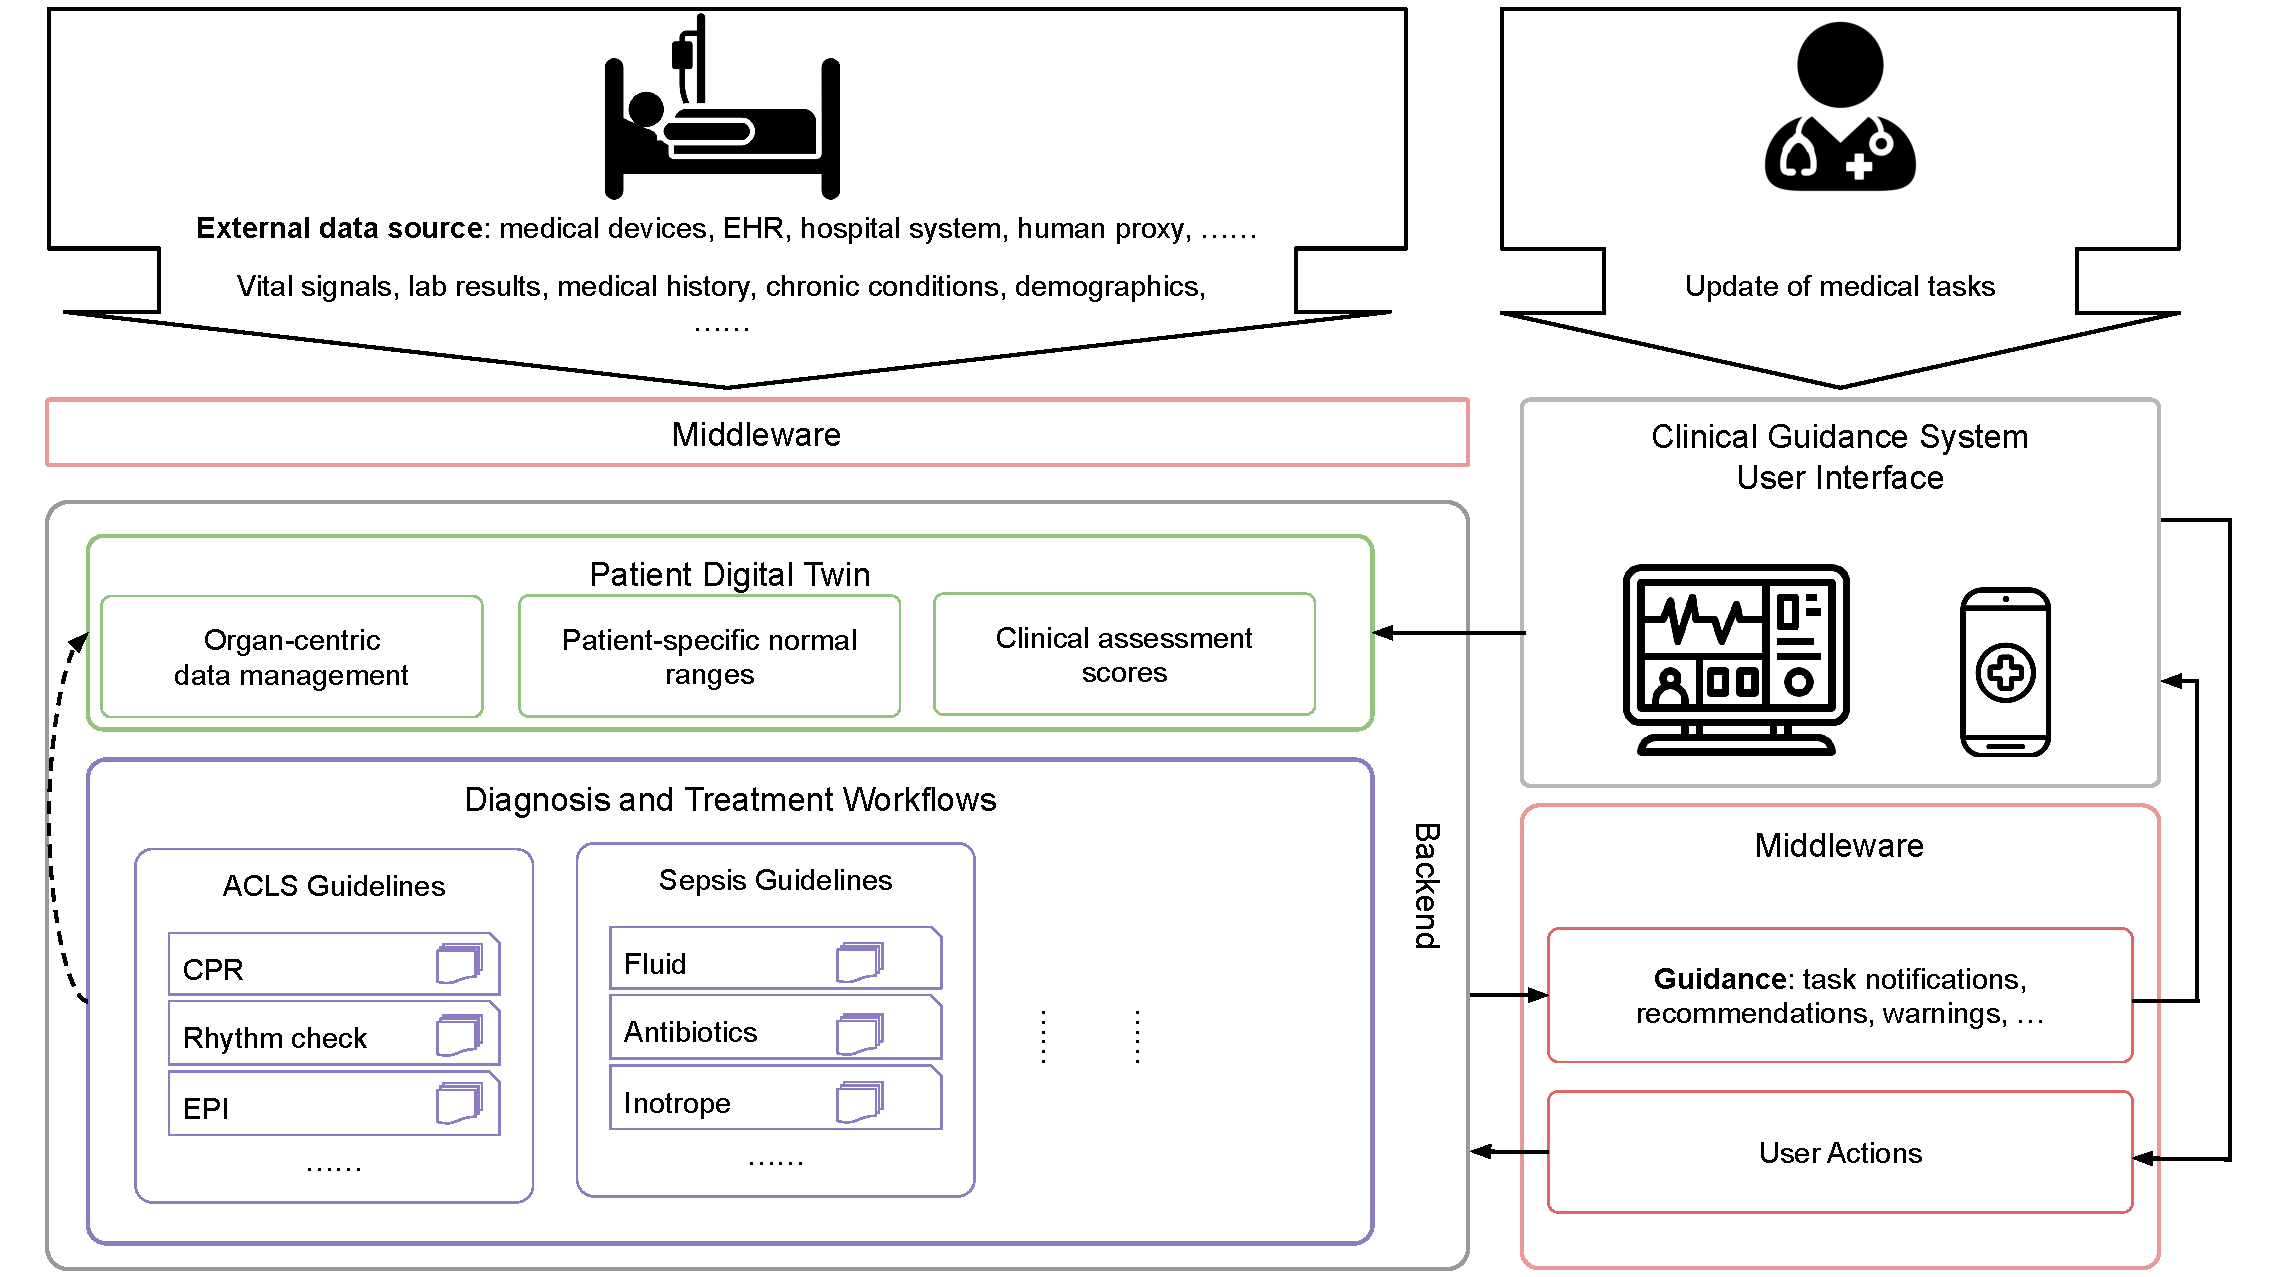
\includegraphics[width=0.95\textwidth]{architecture}
\caption{\CDSSs{} Components}\label{fig:architecture}
\end{figure}


\subsection{Frontend}\label{sec:frontend}

The frontend is the user-facing component of a \CDSS{}, and
handles interactions with users by collecting user actions,
delivering guidance, and displaying data and information.
Ideally a \CDSS{} frontend must be customizable according to
user preferences. As these changes don't directly
affect the underlying medical knowledge, they should remain
\emph{localized} to the frontend itself.
Thus, the architecture shown in \autoref{fig:architecture},
and many implementation from \autoref{chapter:related-work},
compartmentalize the frontend into a standalone component that
can permit adaptions to accommodate user and hospital-specific
preferences that remain isolated to the frontend itself.

Having a modular frontend is also necessitated by increasing
adoption of devices such as phones and tables at medical establishments.
Thus, frontends for modern \CDSSs{} further need to accommodate
diversity in devices, such as phones, portals at patient's bedside, etc.,
and the associated data entry methods, such as digital keyboards, voice
assistants, etc. Thus, a modular, self-contained frontend is
critical to solving problems with modern \CDSS{} implementations.

\subsection{Backend}\label{sec:backend}

Conceptually, the part of the system that encodes the \BPG{}
constitutes what we call the \emph{backend}. \autoref{fig:architecture}
depicts these as treatment workflows.
In practice, however, the backend can be intertwined with other components in a
monolithic system, be implemented as a shareable,
standalone component, or be something in between. Moreover,
the \emph{computable encoding} may not resemble a traditional
non-executable \BPG{}.

As mentioned in \autoref{chapter:hurdles-cdss-adoption}, having
high-quality, guidelines with mechanism that enable systematic
validation of content and ease of sharing is vital to wider
adoption. This work argues that this is enabled through
the use of computer-interpretable guidelines that can serve as
both textual \BPGs{} and their computer interpretable counterparts. Thus,
ideally, the backend should comprise of a computer-interpretable guideline.

In \autoref{chapter:related-work}, we introduced existing approaches
for expressing guidelines in a computer-interpretable manner.
As discussed in \autoref{sec:related-work-discussion}, several
approaches also stress on using formal methods-based techniques to further
ensure system correctness. Thus, good \BPGs{}, and
their computer-interpretable translations, require significant
effort to develop and verify. This cost can be
be offset by ensuring that the backend can be shared
across \CDSSs{} implementations. Thus, in this work, we
build \CDSSs{} using an architecture where the backend
is a \emph{standalone} component that be composed with
setting-specific frontends to build customizable but safe \CDSSs{}.
By standalone, we specifically mean that the backend should be isolated
such that any changes to any other  component of the \CDSSs{}
should not percolate to the backend itself.


\subsection{Middleware/Additional Infrastructure}\label{sec:middleware}

\autoref{sec:frontend} and \autoref{sec:backend} talk about
the importance of ensuring that conceptually different components are
also implemented and maintained as completely \emph{independent} entities
in practice. This modularity necessitates the need for additional
\emph{glue code} to tie components in a functioning system. For example,
a frontend and backend implemented completely independently of each
other, in unrelated languages, require standardized communication
protocols. Moreover, as \CDSSs{} rely on a diverse spectrum of devices for
data, such as patient health records, real-time monitors and sensors, additional
code has to be written to connect the data to places where it's used in
the backend and frontend.

In this work, we refer to any additional code outside the frontend and
backend as the \say{middleware} or \say{additional infrastructure}.
Note that we use either term interchangeably throughout this work.
Additionally, as shown in \autoref{fig:architecture},
we try to \emph{organize} patient
data into \emph{digital twins} of organ systems whenever applicable.
Notionally, we use \say{digital twins} as virtual entities that encapsulate
actual physical processes or objects,
as is typical in modeling and simulation \cite{TaoJMS22}.
In practice, however, we recognize that such abstractions may be
imprecise, due to differences between \CDSSs{} and traditional
closed-loop systems discussed at the start of this chapter. Thus,
digital twins in our context may simply be simple structures that
hold linked data. For example, while we may notionally refer to an abstract data type
used to record a patient's heart rate and blood pressure as a digital twin of
the patient's cardiovascular system, such a twin would be a very incomplete
representation of the patient's actual cardiovascular system.

